\documentclass{beamer}
%\documentclass[dvips]{beamer}

\mode<presentation>
\usetheme{Warsaw}
\usecolortheme{dolphin}

\usepackage[utf8]{inputenc}
\usepackage[czech]{babel}
\usepackage{xcolor}
\usepackage{graphicx}
\usepackage{caption}
\usepackage{subcaption}
\usepackage{verbatim}
\usepackage{hyperref}
%\usepackage{cite} % pokud je nastaven nejde citovat :-)

\setbeamercovered{transparent}
\setbeamertemplate{bibliography item}[text]
\setbeamertemplate{caption}[numbered] 
\setbeamertemplate{footline}[frame number]
\setbeamertemplate{blocks}[rounded][shadow=true]

\pgfdeclareimage[height=0.8cm]{CVUTlogo}{logo_cvut}
\logo{\pgfuseimage{CVUTlogo}}

%-----------vlastni barvy-------------
\definecolor{myGreen}{RGB}{28,142,28}


\title[Clondike]{Clondike}
\author[Novy]{Zden\v{e}k Nov\'{y}}
\institute[FIT]{\small{Vedouc\'{i} pr\'{a}ce: Josef Gattermayer}\\
\vspace{2mm}
\em{Fakulta informačních technologií\\
České vysoké učení technické v Praze}\\
}
\date{\today}
\titlegraphic{
\includegraphics[height=1.3cm]{logo_cvut}}


\begin{document}
\frame{\titlepage}

\section*{Obsah}
\frame{
	\frametitle{Přehled}
	\tableofcontents
}


\mode<handout:0>{\AtBeginSection{\frame{\tableofcontents[currentsection]}}}
%\mode<handout:0>{\AtBeginSubsection{\frame{\tableofcontents[currentsubsection]}}}


\section{Co je Clondike}
\subsection {Hádanka}
\begin{frame}
	\frametitle {Co je Clondike}
	\framesubtitle {Hádanka}
	\setbeamercovered {transparent}
	\begin{block}{Clondike: }
		\begin {columns}[t]
			\begin {column}{9cm}
				\begin {enumerate}
					\item<1,3-> je část státu Aljaška v Severní Americe
					\item<1,5-> je aplikace pro OS Mac zrychlující jeho animace
					\item<1,7-> je nový typ clusteru nad Linuxovými stroji
					\item<1,9-> je freewarová internetová hra typu Solitaire
					\item<1,11-> je aplikace pro hledání zlata a ukládání jeho stavu ve světě
				\end {enumerate}
			\end {column}
			\begin {column}{2cm}
				\setbeamercovered{invisible}
				\begin {itemize}
					\item<4->[] NE
					\item<6->[] NE
					\item<8->[] ANO
					\item<10->[] NE
					\item<12->[] NE
				\end {itemize}
			\end {column}
		\end {columns}
	\end{block}
\end{frame}

%----------------------------------------------Pojmy----------------------------------------------
\subsection{Pojmy}
\begin {frame}
\frametitle {Pojmy - cluster}
	\begin {block} {Cluster}
		Cluster je seskupením volně vázaných počítačů, které spolu úzce spolupracují, takže navenek mohou vypadat jako jeden počítač.\cite{clanekClondike}
	\end {block}
	\begin {block} {Nededikovaný cluster}
		Neexistuje jeden hlavní počítač (správce), takže všechny počítače jsou rovnocenné. Každý počítač může být odpojen, aniž by byl systém narušen nebo ohrožen. Jinak též P2P cluster.\cite{clanekClondike}
	\end {block}
\end {frame}


\begin {frame}
\frametitle {Pojmy - Uzly}
	\begin {block} {Uzel}
		Jedná se o běžící operační systém.\\
		Obyčejně je uzel fyzický počítač, ovšem pro účely testování používáme virtualizaci, kdy na jednom libovolném hostujícím operačním systému běží několik stanic tvořící cluster. \cite{dpAndrejs}
	\end {block}
	\begin {block} {Domovský uzel}
		Počítač, na kterém byl proces spuštěn.
	\end {block}
	\begin {block} {Hostitelský uzel}
		Počítač, na který byl proces migrován.
	\end {block}
\end {frame}

%comment
\begin{comment}
\begin {frame}
\frametitle {Pojmy - Uživatelé 1}
	\begin {block} {Administrátor clusteru}
		Přestože se jedná o nededikovaný cluster, může existovat někdo, kdo rozhoduje o tom, kdo se smí připojit, kdo může migrovat apod.
	\end {block}
	\begin {block} {Uživatel clusteru}
		Osoba, které je zapojena do clusteru a využívá ho (migruje procesy a dodává výpočetní výkon).
	\end {block}
\end {frame}

\begin {frame}
\frametitle {Pojmy - Uživatelé 2}
	\begin {block} {Administrátor uzlu}
		Administrátor alespoň jednoho uzlu clusteru, který má plný přístup (i fyzický) k uzlu.
	\end {block}
	\begin {block} {Lokální uživatel uzlu}
		Uživatel uzlu, který není uživatelem clusteru.
	\end {block}
\end {frame}
\end{comment}
%end comment

%----------------------------------------------Definice-----------------------------------
%\section{Co je Clondike}
\subsection {Definice}
\begin{frame}
\frametitle{Co je Clondike}
\framesubtitle{Definice}
\setbeamercovered {dynamic}%budou zašedlé
	Clondike:
	\begin {itemize}
		\item je projekt vyvíjený na ČVUT v Praze (FEL, FIT)
		\pause
		\item je nový typ nededikovaného clusteru nad Linuxovými stroji
		\item jeho výpočetní jednotky jsou obyčejné Linuxové pracovní stanice
		\pause
		\item vytváří iluzi jednoho výkonného systému
		\begin {itemize}
			\item SSI - Single system image
		\end{itemize}
		\pause
		\item jeho stanice mohou být integrovány jen částečně
	\end{itemize}
\end{frame}


\begin{frame}
\frametitle{O čem jsem mluvil???}
	\begin {center}
		
\includegraphics[height=5cm]{otaznik}
	\end {center}
\end{frame}
%\section{Co je Clondike}
\begin {frame}
\frametitle{Tak jinak, co to je Clondike?}
	Clondike:
		\begin {itemize}
			\pause
			\item je nástroj ke sdílení výpočetního výkonu počítačů na úrovni procesů
			\pause
			\item umožňuje, aby ostatní počítače "půjčili" svůj hardware počítači, který spouští nějakou složitější úlohu
			\pause
			\item je použitelný pro obyčejné Linuxové stanice
			\pause
			\item nezdržují a nezatěžují uživatele
			\begin {itemize}
				\item fungováním na pozadí
				\item "půjčujováním" hardwaru jen pokud je nevytížený (nastavitelné)
				\item malými nároky na rozdělování a přijímání úloh
			\end{itemize}
		\end{itemize}
\end {frame}

%-------------------------------------------Jak to funguje--------------------------------------------
\section{Jak to funguje}
\begin {frame}
\frametitle{Jak to funguje (1)}
\framesubtitle {Na začátku}
	\begin {figure}
		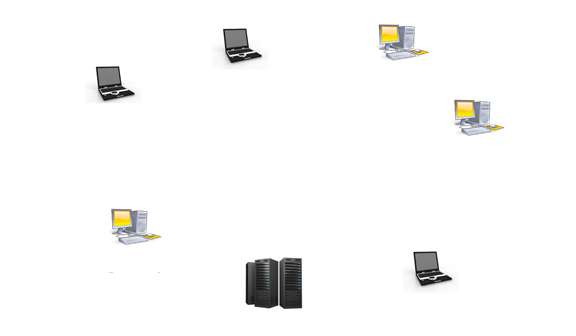
\includegraphics[height=0.7\textheight]{faze0}
		\caption{Počáteční stav}
	\end {figure}
\end {frame}

\begin {frame}
\frametitle{Jak to funguje (2)}
\framesubtitle {Vytvoření úlohy}
	\begin {figure}
		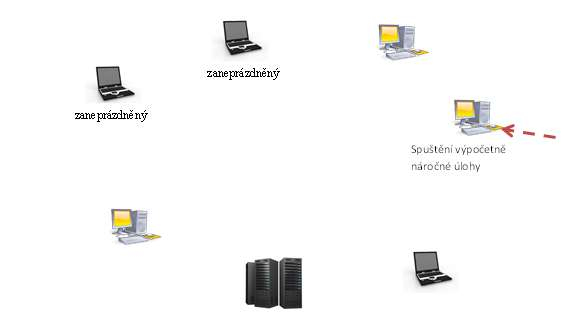
\includegraphics[height=0.7\textheight]{faze1}
		\caption{Vytvoření úlohy počítačem}
	\end {figure}
\end {frame}

\begin {frame}
\frametitle{Jak to funguje (3)}
\framesubtitle {Sdílení úlohy mezi nečinné stanice}
	\begin {figure}
		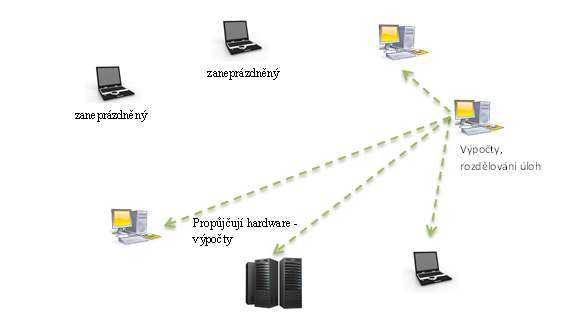
\includegraphics[height=0.7\textheight]{faze2}
		\caption{Rozdělení úlohy mezi nečinné stanice}
	\end {figure}
\end {frame}

\begin {frame}
\frametitle{Jak to funguje (4)}
\framesubtitle {Změna stavu některých stanic}
	\begin {figure}
		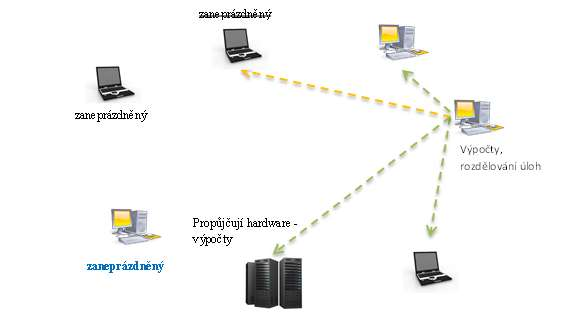
\includegraphics[height=0.7\textheight]{faze3}
		\caption{Přerozdělení úlohy}
	\end {figure}
\end {frame}

%----------------------------------------Mechanismus migrace-----------------------------------------
\begin {comment}
\section {Mechanismus migrace}
\begin {frame}
\frametitle {Mechanismus migrace procesu}
	Domovský uzel:
	\begin {enumerate}
		\item pozastavení procesu - přepnutí do migračního módu
		\item zavření dosud oteřených souborů
		\item vytvoření checkpointu %prozatimní uložený stav
		\item přenos checkpointu na cílový uzel
	\end {enumerate}
	Hostitelský uzel:
	\begin {enumerate}
		\item otevření potřebných souborů
		\item spuštění procesu z checkpointu
	\end {enumerate}
\end {frame}
\end {comment}

\section {Clondike nyní a moje úloha v něm}
\begin {frame}
\frametitle {Clondike nyní}
	\begin{block} {Nynější stav:}<1>
		\begin{itemize}
			\item na projektu se po odstávce opět začíná pracovat
			\item nynější verze Clondike funguje v kernelu 2.6.33.1
			\item nynější vývojový tým:
			\begin {itemize}
				\item 1 student -- disertační práce
				\item 1 student -- diplomová práce
				\item 3 studenti -- bakalářská práce
			\end {itemize}
			
		\end {itemize}
	\end {block}
	\begin {block} {Úkol}<2>
				Vytvořit \alert{patch} Clondike, aby fungoval na kernelu 3.X, dodělat dokumentaci a případně vylepšit plánovač procesů.
	\end {block}
\end{frame}	

\begin{frame}
\frametitle {Já a Clondike}
	\begin{block} {Moje role v projektu:}
		\begin{itemize}
			\item testování a měření
			\item úprava a tvorba dokumentace
			\item rešeršní studie open source hostingu pro kódy
			\item založení a správa hostingu kódů a dat
			\item poskytnutí technické podpory ostatním vývojářům
		\end{itemize}
	\end  {block}
\end{frame}


\section {Příklad použití}
\subsection {Instituce}
\begin{frame}
\frametitle{Příklad použití v instituci}
\setbeamercovered {dynamic}
	\begin {exampleblock} {Problém}
			\begin{itemize}
				\item velká instituce (firma, škola) s mnoha počítači
				\item většina počítačů výkonostně naddimenzována
				\item nárazové používání těchto počítačů
				\item na několika počítačích probíhají složité (časově náročné) výpočty
			\end{itemize}
	\end{exampleblock}
	\pause
	\begin {exampleblock} {Řešení}
		\alert {Clondike}	
	\end {exampleblock}
\end{frame}

\subsection {Přátelé}
\begin{frame}
\frametitle{Příklad použití mezi přáteli}
\setbeamercovered {dynamic}
	\begin {exampleblock} {Problém}
			\begin{itemize}
				\item skupina přátel chce vzájemně sdílet výpočetní výkon
				\item každý provádí složité výpočty jindy
			\end{itemize}
	\end{exampleblock}
	\pause
	\begin {exampleblock} {Řešení}
		Díky P2P architektuře:\\
		\alert{Clondike}
	\end {exampleblock}
\end{frame}

%--------------------------------------------zdroje----------------------------------------------
\mode<handout:0>{\AtBeginSection{}}

\appendix
\section<presentation>{Zdroje}
%\subsection<presentation>*{Bibliografie}
\begin{frame} [allowframebreaks]
  \frametitle<presentation>{Zdroje}
  \begin{thebibliography}{9}
    %  \beamertemplatebookbibitems 
	\bibitem{dpMalat}{\em MALÁT, Petr.}
		{\bf Podpora vícevláknových aplikací v projektu Clondike}
		[online]. Praha, 2010 [cit.~2012-11-01]. Diplomová práce. Fakulta elektrotechnická, České vysoké učení technické v~Praze. Vedoucí práce Mgr. Martin Štava. Dostupné z: \url{https://dip.felk.cvut.cz/browse/pdfcache/malatpe1_2010dipl.pdf}.

	\bibitem{dpAndrejs}{\em ANDREJS, Pavel.}
		{\bf Implementace bezpečnostních mechanismů pro Clondike}
		[online]. Praha, 2009 [cit.~2012-11-01]. Diplomová práce. Fakulta elektrotechnická, České vysoké učení technické v~Praze. Vedoucí práce Ing. Martin Kačer, Ph.D. Dostupné z: \url{https://dip.felk.cvut.cz/browse/pdfcache/andrep1_2009dipl.pdf}.

	\bibitem{clanekClondike}{\em GATTERMAYER, Josef a Michal ŠŤAVA.}
		{\bf Parallel Computing Group: Clondike}
		[online]. 2008, č.~1, 2011-11-19 [cit.~2012-11-01]. Dostupné z: \url{http://pcg.fit.cvut.cz/structure/clondike}.

	\bibitem{mozilla}{\em MOZILLA EUROPE a MOZILLA FOUNDATION.}
	{\bf Mozilla Firefox 16.0} [software]. [přístup 2.~listopad~2011]. Dostupné z: \url{www.mozilla.org/cs/firefox/}.

	\bibitem{texlive}{\em TUG.}
	{\bf \TeX~live} [software]. [přístup 2.~listopad~2011]. Dostupné z: \url{http://www.tug.org/texlive/}.
  \end{thebibliography}
\end{frame}


%-------------------------------------------Zaver---------------------------------------------
\begin {frame}
\frametitle{Dotazy}
	\setbeamercovered {dynamic}
	\begin {center}
		\huge \textcolor{myGreen}{\textbf{Dotazy?}}\\
		\vspace{12mm}
		\pause
		\huge {Děkuji za pozornost\ldots}
	\end {center}
\end {frame}


\end{document}

